\section{Formato di scambio dei dati}
\label{sec:chapter_architettura_sistema_formato_scambio}

Per permettere la comunicazione delle  tre componenti principali (servizio, editor, navigatore) del sistema creato per il presente lavoro di tesi è stato utilizzato un formato di scambio di dati completamente indipendente dal linguaggio di programmazione: JSON (JavaScript Object Notation).
Questo formato si basa sul linguaggio JavaScript ed utilizza testo, semplice da leggere e scrivere, per trasmettere dati costituiti da coppie attributo-valore (oggetti).
\\
Esso rappresenta il formato  di dati più usato per permettere la comunicazione asincrona tra browser/server, questo perchè utilizza convenzioni conosciute dai programmatori Java, Javascritpt, C, Perl, Python per citarne alcuni. Questa caratteristica rende di fatto il JSON un linguaggio ideale per lo scambio di dati ed ha consentito in questo lavoro la comunicazione tra un’ applicazione browser lato client scritta in Javascript (sia l’ editor che il navigatore) ed il servizio lato server scritto in Python.
\\
Il formato JSON è basato su due strutture di dati universali:
\begin{itemize}
\item Un insieme di coppie nome/valore. In base al tipo di linguaggio utilizzato esse possono rappresentare un oggetto, un record, una struct, un dizionario, una tabella hash, un elenco di chiavi, un array associativo.
\item Un elenco ordinato di valori. Nelle maggior parte dei linguaggi essi rappresentano un array o un vettore.
\end{itemize}

Nello specifico queste strutture vengono rappresentate tramite oggetti, array e valori:
\begin{itemize}
\item Un oggetto è una serie non ordinata di nomi/valori che inizia con una parentesi graffa sinistra e termina con una destra. Ogni nome è seguito dai due punti ed i valori sono separati dalla virgola.
\begin{figure}[htb]
 \centering
 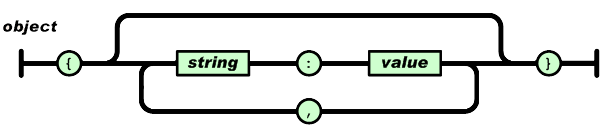
\includegraphics[width=0.9\linewidth]{images/chapter_architettura_sistema/oggetto_json.png}\hfill
 \caption[Un oggetto JSON]{Un oggetto JSON}
 \label{fig:architettura_sistema_oggetto_json}
\end{figure}
\item Un elenco ordinato di valori. Nelle maggior parte dei linguaggi essi rappresentano un array o un vettore.
\begin{figure}[htb]
 \centering
 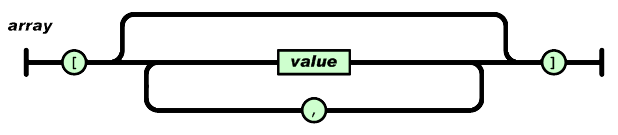
\includegraphics[width=0.9\linewidth]{images/chapter_architettura_sistema/array_json.png}\hfill
 \caption[Un array JSON]{Un array JSON}
 \label{fig:architettura_sistema_array_json}
\end{figure}
\item Un valore può essere di tipo booleano (true, false), un numero (intero, reale o in virgola mobile), una stringa, un oggetto o un array. Queste strutture possono essere annidate.
\begin{figure}[htb]
 \centering
 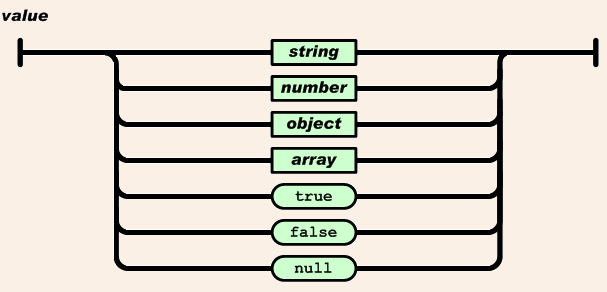
\includegraphics[width=0.8\linewidth]{images/chapter_architettura_sistema/valore_json.png}\hfill
 \caption[Un valore JSON]{Un valore JSON}
 \label{fig:architettura_sistema_valore_json}
\end{figure}

\end{itemize}

Inoltre sono disponibili funzioni, scritte in diversi linguaggi di programmazione tra cui JavaScript e Python, che permettono facilmente di effettuare il parsing e la scrittura del formato dati JSON. Questa caratteristica è stata sfruttata in questo elaborato ed ha agevolato il lavoro di lettura e scrittura del JSON.
Tramite l’utilizzo di queste strutture dati all’interno del JSON è possibile definire il proprio formato di scambio (uno standard), creato appositamente per il trasferimento dei dati voluti.
Three.js definisce infatti il proprio standard tramite due formati differenti: il formato JSON 3 ed il formato JSON 4. 
\\
Entrambi i formati sono stati oggetto di profondo studio nel presente lavoro, questo ha permesso di valutare quale tra i due si addicesse meglio ad essere utilizzato all’interno dell’ecosistema creato. 

\subsection{I due formati di Three.js}
Attualmente in Three.js sono definiti due standard differenti per il trasferimento di dati: il formato JSON 3 e JSON 4. Di fatto questi formati descrivono la metodologia con cui deve essere scritto il file di testo affinché il parser possa riconoscere correttamente le informazioni inserite.
Nello specifico il file utilizzato per lo scambio di dati risulta differente in base a quale dei due formati è stato scelto, inoltre ad ogni formato corrisponde uno specifico parser che viene utilizzato per analizzare il testo.
\\
In Three.js risultano già definiti due differenti parser in grado di analizzare i formati JSON 3 e JSON 4. I due analizzatori presentano caratteristiche differenti, che verrano dettagliate successivamente. Inoltre entrambi i formati ed i corrispettivi parser risultano incompleti in quanto non permettono di trasferire alcune strutture dati Three.js, essenziali per questo lavoro di tesi.
Nel presente lavoro inoltre entrambi i formati di scambio sono stati studiati accuratamente per permettere di scegliere quali tra i due meglio si addicesse per l’architettura client/server sviluppata.
\\
In particolare Three.js ha un parser JSON 3 che permette di analizzare (un importer) un formato di questo tipo ma non di scriverlo (un exporter), mentre Blender presenta dei plug-in che permettono di utilizzare un parser sia per la lettura che per la scrittura.
\\
Invece per quanto riguardo il formato JSON 4; Three.js ha un parser che ne permette sia la lettura che la scrittura , mentre Blender ha un plug-in che permette di utilizzare il parser per la sola scrittura di questo formato.
\\
La scelta di quale formato utilizzare è risultata quindi fondamentale al fine di comprendere cosa sviluppare per permettere lo scambio completo dei dati da Three.js verso Blender e da Blender verso Three.js.
Con il formato JSON 3 era necessario creare un exporter scritto nel linguaggio Three.js, mentra con il formato JSON 4 era necessario creare un importer in Blender scritto con il linguaggio Python.
Quest’ultima  tra le due risultava la soluzione più complessa da realizzare in quanto necessitava lo studio di una libreria completamente nuova (quella di Blender) scritta in Python.
Nonostante la maggiore complessità questa soluzione è stata quella adottata in quanto il formato JSON 4 , rispetto al JSON 3, meglio si addiceva al contesto di questo lavoro.
\\
In questo capitolo verranno quindi esaminati i vantaggi e gli svantaggi dei due formati e dei rispettivi parser, verrà inoltre motivata la scelta che ha portato all’utilizzo di un formato piuttosto che di un’altro e verranno descritte le modifiche ed i miglioramenti apportati al formato scelto.

\subsection{Il formato JSON 3}
Il formato JSON 3 permette il trasferimento di dati Three.js attraverso un file di testo molto difficile da scrivere e da leggere. 
Questa difficoltà si ripercuote direttamente sul parser, rendendolo di fatto molto complesso e poco modificabile.
Durante il presente lavoro di tesi è stato confermato che il formato JSON 3 verrà presto deprecato in favore del nuovo formato JSON 4.
\\
Nonostante questo, studiare i vantaggi e gli svantaggi del formato JSON 3 si è reso necessario per poter prendere alcune importanti decisioni progettuali, descritte nell'introduzione al capitolo.
Viene adesso fornito un piccolo esempio di file scritto nel formato JSON 3 in cui vengono riportate le informazioni di due piani (uno blu ed uno rosso) insieme ai corrispondenti parametri di renderizzazione.

\begin{lstlisting}[language=json]
{ 
	"metadata" :{"formatVersion" : 3.1},
	"materials" : [{
		"DbgColor" : 15658734,
		"DbgIndex" : 0,
		"colorDiffuse" : [0, 0, 1],
		"shading" : "Lambert",
		"transparency" : 1.0,
		"trasnparent" : true,
	},{
	"materials" : [{
		"DbgColor" : 15658734,
		"DbgIndex" : 1,
		"colorDiffuse" : [1, 0, 0],
		"shading" : "Lambert",
		"transparency" : 0.5,
		"trasnparent" : true,
	}],
	"vertices" : [1,0,1,1,0,-1...],
	"normals" : [0.1.0],
	"uvs" : [],
	"faces" : [34,0,1,2,0,0,0,0, 34,3,0,2,0,0,0,0, ...]
}
\end{lstlisting}
I parametri fondamentali (visibili nell’esempio) sono:
\begin{itemize}
\item \texttt{materials}: un array di materiali da assegnare ai corrispondenti oggetti dove per ogni materiale vengono descritte le proprietà da esso possedute.
\item \texttt{vertices}: un array di vertici descritti in coordinate mondo. All’interno di questo array sono presenti i vertici di tutti gli oggetti nella scena da renderizzare.
\item \texttt{normals}: un array in cui vengono inserite le normali. Ogni normale è un vettore rappresentato mediante i tre valori (x,y,z). All’interno di questo array sono presenti le normali di tutti gli oggetti nella scena.
\item \texttt{colors}: un array in cui sono descritti i colori delle facce di ogni oggetto presente nella scena.
\item \texttt{uvs}: un array che contiene le coordinate uv di ogni oggetti della scena.
\item \texttt{faces}: un array complesso in cui sono riportate le informazioni di tutte le facce degli oggetti nella scena. In questo array sono presenti dei codici univoci che permettono di descrivere la tipologia di tutte le facce inserite.
\end{itemize}

Il parametro faces risulta il più complesso tra quelli presentati e proprio da quest’ultimo il parser inizia ad analizzare il JSON.
Questo formato si basa infatti sull’utilizzo di una complessa bitmask che permette al parser, a partire dai codici univoci presenti nell’array faces, di riconoscere il numero di vertici che compongono le facce e le caratteristiche che esse possiedono. 
Il codice univoco viene prelevato, convertito in  binario e poi sovrapposto sulla bitmask.
\\
La bitmask utilizzata è la seguente:
\begin{itemize}
\item $00 00 00 00$ = \texttt{TRIANGLE} (3 valori)
\item $00 00 00 01$ = \texttt{QUAD} (4 valori)
\item $00 00 00 10$ = \texttt{FACE\_MATERIAL} (1 valore)
\item $00 00 01 00$ = \texttt{FACE\_UV} (1 valore)
\item $00 00 10 00$ = \texttt{FACE\_VERTEX\_UV} (3 valori se triangolo, 4 altrimenti)
\item $00 01 00 00$ = \texttt{FACE\_NORMAL} (1 valore)
\item $00 10 00 00$ = \texttt{FACE\_VERTEX\_NORMAL} (3 valori se triangolo, 4 altrim.)
\item $01 00 00 00$ = \texttt{FACE\_COLOR} (1 valore)
\item $10 00 00 00$ = \texttt{FACE\_VERTEX\_COLOR} (3 valori se triangolo, 4 altrimenti)
\end{itemize}
Al fine di comprendere meglio il funzionamento della bitmask verrà fornito un esempio:

``faces'' : [34,\textcolor{red}{0,1,2,}\textcolor{blue}{0,}\textcolor{purple}{0,0,0,}    34,\textcolor{red}{3,0,2,}\textcolor{blue}{0,}\textcolor{purple}{0,0,0,}    34,\textcolor{red}{4,5,6,}\textcolor{blue}{1,}\textcolor{purple}{0,0,0,}   34,\textcolor{red}{6,4,5,}\textcolor{blue}{1,}\textcolor{purple}{0,0,0}]
\\
Come riportato precedentemente nell’array faces sono rappresentate le diverse facce che compongono l’oggetto da renderizzare.
Ogni faccia è descritta medianti diversi valori nell’ array, il numero di valori dell’array da assegnare alla faccia e cosa rappresentano questi valori viene indicato dal codice univoco in questo caso 34.
\\
Nell’esempio infatti il codice 34 viene convertito nel binario 00100010 e poi sovrapposto sulla bitmask. La sovrapposizione viene effettuata bit a bit a partire da destra verso sinistra.
Nell’ ordine da destra verso sinistra avvengono quindi le seguenti tre sovrapposizioni con il binario 00\textcolor{purple}{1}000\textcolor{blue}{1}\textcolor{red}{0}:

\begin{itemize}
\item \texttt{Triangle} (primo zero a partire da destra): la faccia quindi è costituita da tre vertici (in rosso nell'esempio) e rappresenta quindi un triangolo e non un quadrato. Siccome è la prima sovrapposizione nell’array faces i tre valori dopo il codice rappresentano tre indici da utilizzare nell’array vertices.
\item \texttt{Face Material} (primo uno a partire da destra): alla faccia quindi è associato un materiale. Siccome è la seconda sovrapposizione, nell’array faces il valore dopo le tre cordinate (in blu nell'esempio) rappresenta un indice da utilizzare nell’array materials.
\item \texttt{Face Vertex Normal} (secondo uno a partire da destra): alla faccia sono associate delle normali di vertice. Siccome è la terza sovrapposizione i 3 valori dopo l’indice del materiale (in viola nell'esempio) rappresentano le normali di vertice. La prima normale è associata al primo vertice, la seconda normale al secondo vertice e la terza normale al terzo vertice.
\end{itemize}

Le tre sovrapposizioni calcolate permettono di indicare al parser il numero di indici (oltre al codice) da considerare per la faccia in base al codice ad essa assegnato, in questo caso 7 (3+1+3). 
Questo permette di fatto al parser di distringuere le diverse facce presenti nell’array.
I vertici, nel punto 1, vengono prelevati dall’array vertices grazie agli indici (rossi nell’esempio) inseriti dopo il codice. Ad esempio se l’indice è uguale a 0 vengono prelevati i tre valori a partire dalla posizione zero, mentre se l’indice è uguale ad 1 vengono presi i tre valori a partire dalla posizione tre. Essi rappresentano infatti, nell’ ordine, il valore della coordinata (x, y, z).
Stesso discorso per il punto 2 dove le normali nell’array normals sono prelevate a triplette.
\\
Viene ora fornito un ulteriore esempio, in cui vengono utilizzate facce quadrangolari invece che triangolari. Inoltre viene esaminata la modalità di utilizzo dell’array colors.
\\
Il codice inserito nell' array faces per questo esempio è 65.

\begin{lstlisting}[language=json]
{ 
"metadata" : { "formatVersion" : 3 }, 
"materials" : [], 
"vertices" : [ -5,5,-5, -5,-5,-5, 5,-5,-5, 5,5,-5, -5,5,5, -5,-5,5, 5,-5,5, 5,5,5 ], 
"faces" : [ 65,3,2,1,0,0, 65,4,5,6,7,1, 65,7,6,2,3,2, 65,0,1,5,4,3, 65,0,4,7,3,0, 65,6,5,1,2,1 ], 
"colors": [ 16711680, 65280, 255, 16776960 ], 
"normals": [], 
"uvs": [] 
}
\end{lstlisting}

Anche per questo esempio verrà analizzata una faccia dell'array faces = [65,\textcolor{red}{3,2,1,0,}\textcolor{blue}{0}].
\\
Il codice viene convertito nel binario 01000001 e sovrapposto sulla bitmask.
Nell’ ordine da destra verso sinistra avvengono due sovrapposizioni con il binario 0\textcolor{blue}{1}00000\textcolor{red}{1}:

\begin{itemize}
\item \texttt{Quad}(primo uno a partire da destra): la faccia quindi è costituita da quattro vertici e rappresenta quindi un quadrato e non un triangolo. Siccome è la prima sovrapposizione nell’array faces i quattro valori dopo il codice rappresentano tre indici da utilizzare nell’array vertices.
\item \texttt{Face color} (secondo uno a partire da destra): alla faccia è associato un colore descritti nel formato decimale; in questo caso 16711680 = 0xff0000. Siccome è la seconda sovrapposizione il valore dopo i quattro vertici rappresenta l’indice da utilizzare per prelevare il colore della faccia dall’array colors.
\end{itemize}
Le due sovrapposizione calcolate permettono di indicare al parser che il numero di indici oltre al codice da considerare per la faccia sono 5 (4+1). 
\\
La trattazione del JSON 3 nel presente paragrafo non è volutamente esaustiva ma risulta particolarmente adatta per mostrare i problemi che derivano dall’utilizzo di questo formato di scambio.
\\
Lo standard risulta infatti molto complesso sia da scrivere che da leggere, complessità che aumenta esponenzialmente all’incrementare del numero di oggetti presenti nella scena.
\\
Siccome viene utilizzato un array di vertici ed uno di facce per tutti gli oggetti, tali array con l’incrementare del numero oggetti diventano talmente popolati da risultare di fatto incomprensibili. Per una persona che legge questo formato risulta difficile comprendere non solo quanti e quali oggetti sono presenti nella scena ma anche a quali oggetti associare i parametri di rendering. 
Questo rende difficile modificare a mano un file di testo scritto tramite questo formato.
\\
Inoltre il fatto che tutto sia scritto all’interno di questi array non permette di riportare all’interno del formato di scambio la descrizione gerarchica degli oggetti presenti nella scena.
Descrizione però fondamentale per questo elaborato al fine di mantenere inalterata la scena durante lo scambio di informazioni tra editor e servizio. 
\\
La gerarchia permette alle persone che utilizzano il sistema creato in questo lavoro di tesi di abbracciare un approccio iterativo incrementale. infatti se venisse salvata una scena nel formato JSON 3 e poi quest’ultimo venisse caricato, tutta la gerarchia associata agli oggetti andrebbe persa. Inconveniente non voluto in quanto la scena salvata deve risultare assolutamente identica a come è stata creata.
\\
Infine il parser del JSON 3, descritto in [riferim], risulta non solo molto complesso ma anche poco modificabile. La modificabilità del parser in questo lavoro di tesi risulta però essenziale per inserire nuove informazioni all’interno del file .json. Informazioni che permettono sia di aggiungere parametri del linguaggio Three.js non ancora inseriti nelllo standard JSON (lo standard è infatti incompleto) sia di aggiungere caratteristiche completamente nuove.
\\
Quindi la complessità di questo formato, la totale assenza di gerarchie e la bassa modificabilità del parser hanno fatto propendere la scelta verso il formato JSON 4.

\subsection{Il formato JSON 4}
\label{sec:formato_scambio_formato_json4}

Il formato di scambio JSON 4 descrive i dati Three.js all’interno di un file di testo di più semplice lettura e scrittura rispetto al JSON 3.
\\
In questo formato è inoltre completamente assente la complicata logica basata sulla bitmask.
Una differenza fondamentale rispetto al JSON 3 è la presenza di una descrizione gerarchica degli oggetti nella scena. Vengono infatti descritte esplicitamente le relazioni padre-figlio, relazioni fondamentali all’interno del linguaggio Three.js in quanto permettono la creazione di scene complesse e di oggetti composti.
\\
La gerarchia prevede che tutte le trasformazioni effettuate sul padre si riversino anche sui figli; quindi se un oggetto A è padre di un oggetto B e viene applicata una traslazione ad A, la medesima traslazione viene applicata anche su B. 
\\
L’utilizzo del JSON 4 ha quindi permesso di mantenere inalterata la scena durante il passaggio editor-servizio, cosa che nel formato JSON 3 non sarebbe stato possibile effettuare in quanto tutte le informazioni gerarchiche vengono perse. 
\\
Inoltre ha permesso di inserire un oggetto fittizio come padre dell’ intera scena, agevolando in questo modo le trasformazioni comuni a tutti gli oggetti presenti in essa. 
Ad esempio la rotazione sull’intera scena, invece di avvenire su ogni oggetto che essa contiene, è sufficiente eseguirla sull l’oggetto fittizio.
L’utilizzo di questo oggetto inoltre permette, a chi utilizza il sistema creato nel presente lavoro di tesi, di importare ed assemblare agevolmente più scene differenti provenienti da differenti JSON 4. 
\\
Viene adesso fornito un piccolo esempio di file scritto nel formato JSON 4 in cui vengono riportate le informazioni di due piani insieme ai corrispondenti parametri di renderizzazione.



\begin{lstlisting}[language=json]
{
    "object": {
        "uuid": "AA27DD33-63C4-49D4-ACE4-3850318F6F21",
        "type": "Scene",
        "name": "Scene",
        "matrix": [1,0,0,0,0,1,0,0,0,0,1,0,0,0,0,1],
        "children": [
            {
                "uuid": "108CB82E-56CF-4E45-8463-767E44F2134D",
                "type": "Mesh",
                "name": "mesh",
                "matrix": [1,0,0,0,0,1,0,0,0,0,1,0,0,0,0,1],
                "geometry": "709E63E2-CD16-4B43-A34C-56FCBB8F488C",
                "material": "3FE7EF3A-5890-4E2E-ACFA-6A42FCEE5A69"
            }]
    },

    "geometries": [
        {
            "uuid": "709E63E2-CD16-4B43-A34C-56FCBB8F488C",
            "type": "BufferGeometry",
            "data": {
                "attributes": {
                    "position": {
                        "itemSize": 3,
                        "type": "Float32Array",
                        "array": [-50,50,0,-50,-50,0,50,50,0,-50,-50,0,50,-50,0,50,50,0]
                    },
                    "normal": {
                        "itemSize": 3,
                        "type": "Float32Array",
                        "array": [0,0,1,0,0,1,0,0,1,0,0,1,0,0,1,0,0,1]
                    },

                    "uv": {
                        "itemSize": 2,
                        "type": "Float32Array",
                        "array": [0,1,0,0,1,1,0,0,1,0,1,1]
                    }
                },
            }
        }],
    "materials": [
        {
            "uuid": "3FE7EF3A-5890-4E2E-ACFA-6A42FCEE5A69",
            "type": "MeshPhongMaterial",
            "color": 16777215,
            "map": "80AD9D92-53C5-4F65-B85E-8425B78FD5C5",
            "lightMap": "8FC68D4F-C786-4180-A1D6-DC4892F35295"
        }],
    "textures": [
        {
            "uuid": "80AD9D92-53C5-4F65-B85E-8425B78FD5C5",
            "name": "",
            "repeat": [1,1],
            "offset": [0,0],
            "image": "B9F5F547-5793-41A0-907E-7BCE625AFB77"
        },
        {
            "uuid": "8FC68D4F-C786-4180-A1D6-DC4892F35295",
            "name": "",
            "repeat": [1,1],
            "offset": [0,0],
            "image": "333E1080-5747-415A-9170-05B8D6A745AD"
        }],
    "images": [
        {
            "uuid": "B9F5F547-5793-41A0-907E-7BCE625AFB77",
            "url": "data:image/jpeg;base64,/9j/...
        },
        {
            "uuid": "333E1080-5747-415A-9170-05B8D6A745AD",
            "url": "data:image/jpeg;base64,/9j/...    
}]
}
\end{lstlisting}


Come è possibile notare i due array vertices e faces caratteristici del JSON 3 sono stati completamente abbandonati in favore di una descrizione ad albero della scena molto più comprensibile.
Inoltre i vertici degli oggetti nel JSON 4 sono descritti in coordinate modello invece che mondo. Proprio per questo ad ogni oggetto, oltre ad vertici che lo costituiscono, viene descritta la matrice di trasformazione che riporta le trasformazioni di traslazione, rotazione e scalatura da eseguire su quell’oggetto.
\\
Come osservabile nell’esempio sopra mostrato, la descrizione gerarchica della scena e gli oggetti presenti in essa risultano facilmente comprensibili anche da chi legge il formato per la prima volta.
\\
Verrano ora analizzati i parametri fondamentali di questo formato:

\begin{itemize}
\item \texttt{Object}: rappresenta la scena vera e propria. Al suo interno sono riportati tutti gli oggetti presenti nella scena insieme alle loro informazioni gerarchiche.
\item \texttt{Geometries}: un array in cui sono inserite tutte le geometrie presenti nella scena. Per ogni geometria vengono descritti gli attributi di cui è costituita.
\item \texttt{Materials}: un array in cui sono inseriti tutti i materiali presenti nella scena. Esattamente come per le geometrie, per ogni materiale vengono descritti gli attributi che lo costituiscono.
\end{itemize}
All’interno di object oltre all’ uuid (un codice univoco nel JSON), il nome, il tipo e la matrice di trasformazione viene anche riportato un array children in cui vengono inseriti tutti gli oggetti direttamente figli della scena.
\\
A sua volta ognuno di questi oggetti contiene gli stessi parametri (coppie) posseduti dall’ object scena più ulteriori nuovi come  material e geometry in cui viene indicato per valore il riferimento alla geometria ed al materiale assegnato ad essi.
\\
Ogni coppia geometry e material ha assegnato per valore un uuid che viene utilizzato come indice di ricerca all’interno, rispettivamente, degli array geometries e materials per permettere individuazione della geometria e del materiale corrispondente.
\\
Inoltre ogni oggetto può avere ulteriori figli che, se presenti, vengono inseriti all’interno dell’ array children.

\begin{itemize}
\item \texttt{Position}: contiene i vertici in coordinata modello dell’oggetto.
\item \texttt{Normal}: descrive le normali dell’oggetto.
\item \texttt{Uv}: descrive le coordinate uv dell’oggetto.
\end{itemize}
L’oggetto position in particolare permette di non utilizzare il complesso concetto della bitmask presente nel formato JSON3.
\begin{lstlisting}[language=json]
"position": {
            "itemSize": 3,
            "type": "Float32Array",
            "array": [-50,50,0,-50,-50,0,50,50,0,-50,-50,0,50,-50,0,50,50,0]
            },
\end{lstlisting}
La coppia array rappresenta l’insieme dei vertici che costituiscono l’oggetto di riferimento. 
Il valore itemsize, nell’esempio uguale a 3, indica che ognuno di questi vertici è costituito da tre valori negli assi (x,y,z).
L’ array, visibile nell’esempio, ha la forma [x,y,z,  x,y,z,  x,y,z…].
\\
Per distinguere ogni singolo vertice, esso viene considerato dal parser come un array bidimensionale del tipo [[x,y,z],[x,y,z],[x,y,z]].
\\
In questo array di vertici, a differenza del JSON 3, sono scritti esplicitamente tutti i vertici di ogni triangolo; vengono ripetuti anche  i vertici comuni.
Inoltre la sequenza di vertici viene scritta secondo l’ordine di renderizzazione del triangolo, a differenza del JSON 3 in cui viene scritta in maniera disordinata.
Scriverli in ordine significa che l’array della facce implicitamente considerato è il seguente [[0,1,2],[3,4,5],[6,7,8],[9,10,11],…,[n-2,n-1,n]]. Ogni valore dell’array bidimensionale rappresenta infatti un triangolo ed ogni valore del triangolo rappresenta un indice che permette l’individuzione del vertice (x,y,z) all’interno dell’array dei vertici.
\\
In questo formato si assume che ogni faccia sia costituita solamente da tre vertici (e non anche quattro) in quanto three.js genera facce triangolari.
Inoltre il fatto che in questo formato le facce siano triangolari e che i vertici siano scritti solamente secondo l’ordinamento di renderizzazione permette non solo di eliminare all’interno del json l’informazione delle facce in quanto ridondante, ma permette anche di eliminare tutta la complessa logica basata su bitmask utilizzata nell’altro formato.
\\
Questa caratteristica ha permesso nell’importer di Blender di importare agevolmente le informazioni di vertici e facce di ogni oggetto.

All’interno dell’array materials sono inserite i materiali presenti nella scena e, come le geometrie, ad ogni materiale sono assegnati i parametri che lo contraddistinguono; ad esempio il nome, il colore ed il tipo.
\begin{lstlisting}[language=json]
"materials": [
        {
        "uuid": "3FE7EF3A-5890-4E2E-ACFA-6A42FCEE5A69",
        "type": "MeshPhongMaterial",
        "color": 16777215,
        "map": "80AD9D92-53C5-4F65-B85E-8425B78FD5C5",
        "lightMap": "8FC68D4F-C786-4180-A1D6-DC4892F35295"
        }],
\end{lstlisting}
Inoltre ad ogni materiale possono essere assegnate delle texture. In questo lavoro di tesi sono state utilizzate maggiormente:
\begin{itemize}
\item \texttt{Diffuse texture}: applicate sugli oggetti creati o inseriti nella scena da chi utilizza l’editor.
\item \texttt{Texture lightmap}: applicate automaticamente sugli oggetti della scena dal processo di bake.
\end{itemize}
Se il materiale possiede una diffuse texture sarà infatti presente nell’oggetto json material la coppia che ha per nome map e per valore un id utilizzato come riferimento per trovare la texture all’interno dell’array textures. 
Se invece il materiale possiede una lightmap sarà presente la coppia con nome lightmap.
\\
Nell’ oggetto texture del json sono descritti gli attributi della texture ed inoltre è presente una coppia con nome \texttt{image} che ha per valore un id da utilizzare come riferimento per trovare i dati dell’immagine vera e propria.
\\
Come osservabile questo formato risulta meno compresso rispetto a quello JSON 3 ma permette una maggiore leggibilità dei dati, fondamentale per questo lavoro. 
\\
Inoltre la maggiore compressione del JSON 3 non comporta grandi benefici in termini di dimensioni del formato di scambio in quanto le informazioni più pesanti come i dati delle texture e dei vertici risultano invariate.
\\
Il JSON 4 quindi è risultato il formato ideale per effettuare lo scambio dei dati. Esso però, esattamente come il formato JSON 3 è lungi dall’ essere completo. 
Molte delle strutture dati presenti in Three.js ancora non hanno una descrizione standardizzata sulla controparte JSON, non permettendo quindi lo scambio di alcuni dati che in questo lavoro di tesi era fondamentale trasferire.
\\
Fortunatamente però il parser del JSON 4, descritto in [riferim], risulta di semplice comprensione e modificabile. Questa caratteristica ha permesso di aggiungere nuovi parametri, definiti appositamente per questo lavoro di tesi, all’interno del json al fine di descrivere le strutture dati mancanti.
\\
Le nuove coppie aggiunte oltre a completare una mancanza dello standard JSON 4, permettendo la mappatura di strutture dati esistenti in Three.js, hanno permesso di descrivere nel JSON le nuove funzionalità uniche dell’ editor creato durante questo lavoro di tesi; funzionalità che l’editor normale Three.js non possiede.


\subsection{Il formato JSON 4 modificato}

Il formato JSON 4 come spiegato nel paragrafo precedente è stato modificato per sopperire alle mancanze dello standard e per aggiungere nuove informazioni create appositamente per questo lavoro di tesi. Le informazioni vengono scritte medianti coppie.
\\
Aggiungere nuove coppie non è un’operazione semplice; bisogna infatti definire un nome univoco e decidere il tipo di valore da assegnargli.
Inoltre oltre a descrivere la coppia, bisogna anche definire all’interno di quale oggetto del JSON questa verrà inserita.
\\
Una volta che la coppia è stata definita, bisogna modificare il parser esistente affinchè esso possa riconoscere o scrivere la nuova coppia quando necessario. 
Le maggiori modifiche ed aggiunte apportate riguardano come le informazioni delle texture vengono riportate all’interno del file .json.
Lo standard prevedeva che le immagini fossero indicate all’interno del JSON solamente tramite il path locale alla texture. Questo avrebbe comportato durante lo scambio di dati l’invio oltre al json anche delle texture utilizzate.
\\
Nel presente lavoro di tesi si è preferito utilizzare però un unico file di scambio che contenesse tutte le informazioni della scena, comprese le immagini, al fine di semplificare la costruzione/modifica dei parser del servizio creato. Infatti sia Three.js che Python offrono funzioni che permettono di scrivere e caricare facilmente immagini codificate secondo questo standard.
Le immagini inserite vengono quindi convertite in base 64, una stringa di caratteri che rappresenta l’immagine , ed inserite direttamente nel file di scambio come valore della coppia url.
\begin{lstlisting}[language=json]
"images": [
        {
        "uuid": "B9F5F547-5793-41A0-907E-7BCE625AFB77",
        "url": "data:image/jpeg;base64,/9j/...
        }
        ]
\end{lstlisting}
Three.js inoltre non riportava le informazioni di repeat associate ad ogni texture. 
Il repeat permette di ripetere più volte una texture, sull’asse x ed y, sulla superficie dell’oggetto a cui è applicata. Questa informazione è essenziale in questo lavoro di tesi per evitare l'applicazione su oggetti di texture allungate che non risulterebbero realistiche.
\begin{figure}[htb]
 \centering
 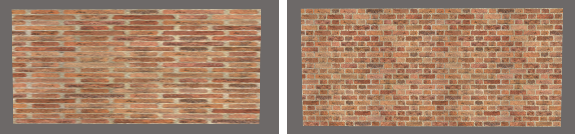
\includegraphics[width=1\linewidth]{images/chapter_architettura_sistema/repeat.png}\hfill
 \caption[Esempio di ripetizione delle texture]{A sinistra una texture non ripetuta, a destra una texture ripetuta quattro volte in orizzontale}
 \label{fig:architettura_sistema_repeat}
\end{figure}
Questa informazione è stata quindi inserita nel JSON all’interno dell’array textures tramite la coppia con nome repeat. 
\\
Ad essa viene assegnato per valore un array di cui il primo elemento rappresenta il valore di repeat sull’asse x, mentre il secondo rappresenta il valore di repeat sull’asse y.
\begin{lstlisting}[language=json]
"textures": [
        {
            "uuid": "80AD9D92-53C5-4F65-B85E-8425B78FD5C5",
            "name": "",
            "repeat": [1,1],
            "offset": [0,0],
            "image": "B9F5F547-5793-41A0-907E-7BCE625AFB77"
        },
],
\end{lstlisting}
Inoltre Three.js non riportava nemmeno l’informazione delle texture env-map di riflessione e rifrazione costruite tramite l’utilizzo di CubeCamera.
\begin{lstlisting}[language=json]
"children": [
    {
        "uuid": "8D7C8218-DBB6-4567-9ED1-160841201F15",
        "type": "CubeCamera",
        "mapping": 301,
        "matrix": [1,0,0,0,0,1,0,0,0,0,1,0,0,0,0,1],
        "children": [
            {
                "uuid": "D2E3E64A-74B7-4391-B57F-D29A1CA64800",
                "type": "PerspectiveCamera",
                "matrix": [-2,0,-1,0,0,-1,0,0,-1,0,2,0,0,0,0,1],
                "zoom": 1,
                "fov": 90,
                "aspect": 1,
                "near": 1,
                "far": 10000
            },
            ...]
    }],
\end{lstlisting}
Le informazioni delle CubeCamera non sono infatti normalmente inserite all’interno del formato di scambio. 
Queste informazioni sono state quindi aggiunte all’interno del formato e sono state sfruttate per permettere lo scambio delle informazioni sulle env-map.
\\
Per ogni CubeCamera nel JSON viene indicato a quale oggetto assegnarla e vengono descritte le informazioni di tutte e sei le perspective camera ad essa assegnate. 
Inoltre è stato creata la coppia mapping per indicare se la cube map deve essere utilizzata per la riflessione o per la rifrazione. La coppia accetta come valore lo stesso id univoco utilizzato in Three.js che risulta differente per la riflessione e rifrazione. Viene utilizzato il valore 301 per la riflessione e 302 per la rifrazione.
\\

Nel formato sono state aggiunte anche le informazioni delle skybox quando essa viene inserita nella scena. La skybox rappresentano l’ambiente (di solito il cielo) che circonda la scena mediante 6 immagini applicate ad un cubo. Risulta quindi chiaro quanto essa fosse fondamentale per ottenere una scena fotorealistica.
Inoltre sono stati inseriti ulteriori parametri non presenti nello standard del formato JSON per permettere di comunicare al servizio ulteriori informazioni.

\begin{lstlisting}[language=json]
"children": [
    {
        "uuid": "57432C9D-67DF-4B43-A536-77BB7645EAFC",
        "type": "Mesh",
        "avoid_bake": true,
        "name": "mesh",
        "matrix": [1,0,0,0,0,1,0,0,0,0,1,0,0,0,0,1],
        "geometry": "D6F14425-4F6C-4D75-974C-02C6B18D07A7",
        "material": "95139D79-876C-4DA6-9AD8-FE8A79B642E2"
    }]
\end{lstlisting}
In questo lavoro di tesi ad ogni oggetto possono essere assegnate due nuove coppie che accettano come valore un booleano:

\begin{itemize}
\item \texttt{Not\_project\_shadow}: quando è true all’oggetto verrà applicata la lightmap, ma esso non influenzerà gli altri oggetti nella scena ( ad esempio non proietta la sua ombra).
\item \texttt{Avoid\_bake}: quando è true permette all’oggetto di evitare completamente il processo di bake. Di fatto all’oggetto non verranno quindi applicate le lightmap ed inoltre non influenzerà gli altri oggetti presenti nella scena.
\end{itemize}
Not\_project\_shadow viene invece utilizzata quando si vuole che un oggetto riceva gli effetti di luce ed ombra dall’ambiente ma che esso non proietti la sua ombra sull’ambiente.
Avoid\_bake invece è utile per nascondere completamente un oggetto dal processo di bake. Questo attributo è stato fondamentale per permettere l’utilizzo di skybox. Per definizione le texture che costituiscono la skybox non devono essere influenzate dalla scena creata. Ad esempio è impensabile che una skybox che rappresenta il cielo possa ricevere ombra.
\\
Inoltre questo parametro quando viene aggiunto ad un oggetto permette di velocizzare il processo di bake in quanto questo oggetto non viene valutato. Quindi può essere utilizzato su quegli oggetti che influenzano poco la scena (ad esempio un libro di una libreria) per migliorare le prestazioni generali del sistema. Questi due attributi verrano approfonditi nel capitolo \ref{cha:chapter_baking_service} .